\chapter{Estabilidade e Controle}
\label{estabilidade}

\section{Diagrama Vn}
\label{diagramavn}

\begin{figure}[H]
\centering
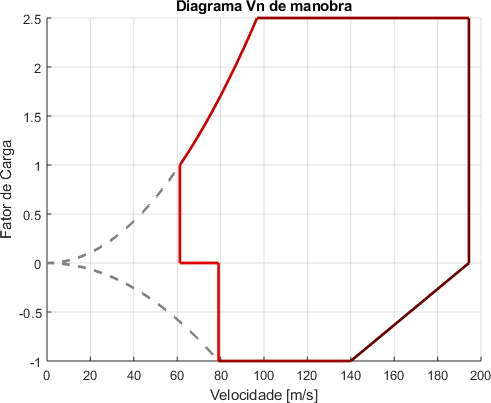
\includegraphics[width=0.75\textwidth]{images/parte3/diagramavn_asalimpa.png}
\caption[Diagrama Vn]{Diagrama Vn}
\label{fig:diagramavn}
\end{figure}

\subsection{Principais Derivadas Longitudinais}
\label{derivadas}

\begin{table}[H]
\centering
\begin{tabular}{cccc}
\toprule
$ \frac{\partial C_{L_{asa}}}{\partial \alpha} $ & 4.586 & $ \frac{\partial C_{L_{eh}}}{\partial \alpha} $ & 3.566 \\ [0.3cm]
$ \frac{\partial C_{L_{eh}}}{\partial \eta} $ & 1.837 & $ \frac{\partial C_{L_{eh}}}{\partial \delta_{tab}} $ & 1.097 \\ [0.3cm]
$ \frac{\partial C_{H_{eh}}}{\partial \alpha} $ & -0.0967  & $ \frac{\partial C_{H_{eh}}}{\partial \eta} $ & -0.4246 \\ [0.3cm]
$ \frac{\partial C_{H_{eh}}}{\partial \delta_{tab}} $ & -0.2015 & $ \frac{\partial \epsilon}{\partial \alpha} $ & 0.1352 \\ [0.3cm]
\bottomrule
\end{tabular}
\caption[Principais Derivadas Longitudinais]{Principais Derivadas Longitudinais}
\label{tbl:derivadas}
\end{table}

\section{Margem Estática Longitudinal}
\label{margem}


\begin{table}[H]
\centering
\begin{tabular}{cc}
\toprule
$ h_n $ & 0.3056 \\
$ h_n' $ & 0.2933 \\
\bottomrule
\end{tabular}
\caption[Ponto Neutro]{Ponto Neutro}
\label{tbl:ponto_neutro}
\end{table}

\begin{table}[H]
\centering
\begin{tabular}{ccc}
\toprule
CG & Traseiro & Dianteiro \\ \midrule
$ K_n $ & 5.56\% & 30.56\% \\
$ K_n' $ & 4.33\% & 29.33\% \\
\bottomrule
\end{tabular}
\caption[Margem Estática Longitudinal]{Margem Estática Longitudinal}
\label{tbl:margem_estatica}
\end{table}

\section{Controle Longitudinal - Profundor}
\label{controlelongitudinal}

\begin{figure}[H]
\centering
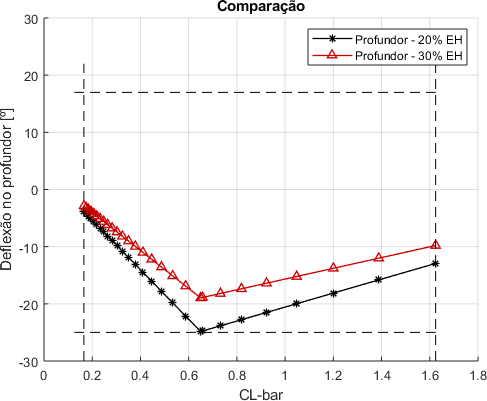
\includegraphics[width=0.75\textwidth]{images/parte3/comparacao_deflexao.png}
\caption[Comparação de Deflexão entre diferentes profundores em tamanho para manobra equilibrada]{Comparação de Deflexão entre diferentes profundores em tamanho para manobra equilibrada no fator de carga máximo e CG dianteiro}
\label{fig:comp_def}
\end{figure}

\begin{figure}[H]
\centering
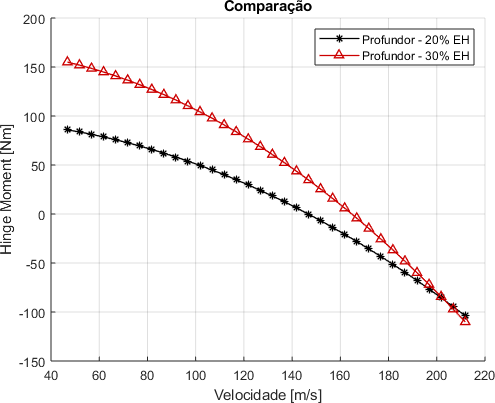
\includegraphics[width=0.75\textwidth]{images/parte3/comparacao_hingemoment.png}
\caption[Comparação de \textit{Hinge Moment} entre diferentes profundores em tamanho]{Comparação de \textit{Hinge Moment} entre diferentes profundores em tamanho para voo reto e nivelado e CG dianteiro}
\label{fig:comp_hingemoment}
\end{figure}


\begin{table}[H]
\centering
\begin{tabular}{ccc}
\toprule
CG & Traseiro & Dianteiro \\ \midrule
$ H_m $ & 12.58\% & 37.72\% \\
$ H_m' $ & 10.52\% & 35.65\% \\
\bottomrule
\end{tabular}
\caption[Margem de Manobra Longitudinal]{Margem de Manobra Longitudinal}
\label{tbl:margem_manobra}
\end{table}

\begin{figure}[H]
\centering
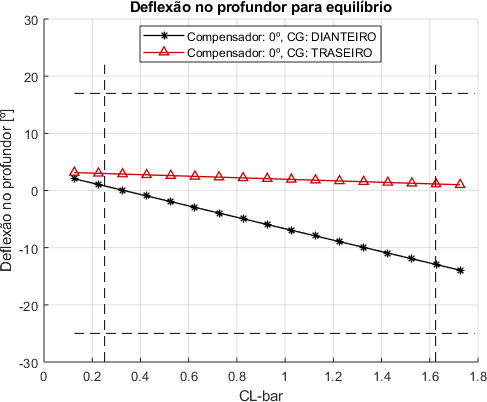
\includegraphics[width=0.75\textwidth]{images/parte3/De_equi_c20.png}
\caption[Deflexão de profundor para voo reto e nivelado]{Deflexão de profundor para voo reto e nivelado}
\label{fig:def_voo1g}
\end{figure}

\begin{figure}[H]
\centering
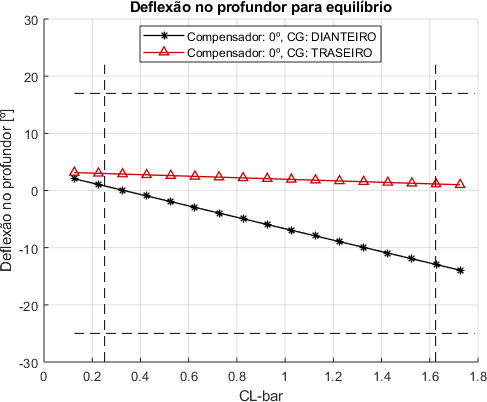
\includegraphics[width=0.75\textwidth]{images/parte3/De_equi_c20.png}
\caption[Deflexão de profundor para voo reto e nivelado]{Deflexão de profundor para voo reto e nivelado}
\label{fig:def_voo1g}
\end{figure}

\begin{figure}[H]
\centering
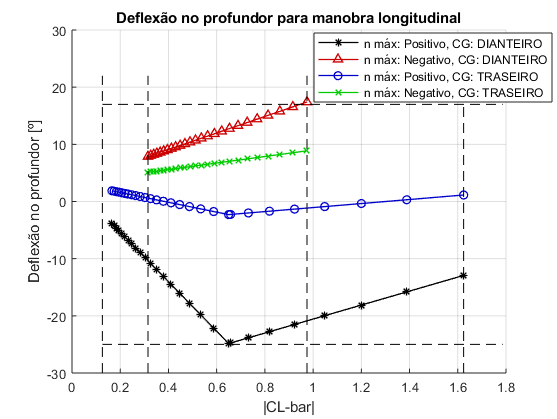
\includegraphics[width=0.75\textwidth]{images/parte3/De_man_c20.png}
\caption[Deflexão de profundor para manobra equilibrada]{Deflexão de profundor para manobra equilibrada}
\label{fig:def_vooNz}
\end{figure}
